% 2023 新高考Ⅰ卷 18：正四棱柱 ABCD-A1B1C1D1，A2/B2/C2/D2 分别在四条侧棱上
% （AA2=1、BB2=DD2=2、CC2=3），P 在棱 BB1 上
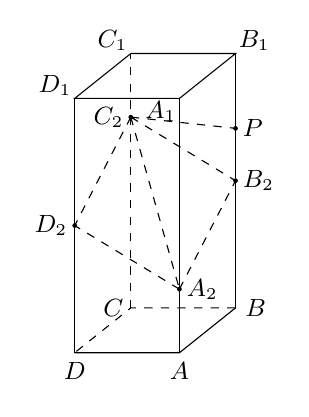
\begin{tikzpicture}[scale=0.95, font=\small]
  \coordinate (D)  at (0,0);
  \coordinate (A)  at (1.4,0);
  \coordinate (B)  at (2.15,0.6);
  \coordinate (C)  at (0.75,0.6);
  \coordinate (D1) at (0,3.4);
  \coordinate (A1) at (1.4,3.4);
  \coordinate (B1) at (2.15,4.0);
  \coordinate (C1) at (0.75,4.0);
  \coordinate (A2) at (1.4,0.85);
  \coordinate (B2) at (2.15,2.3);
  \coordinate (C2) at (0.75,3.15);
  \coordinate (D2) at (0,1.7);
  \coordinate (P)  at (2.15,3.0);
  \draw (D) -- (A) -- (B);
  \draw[dashed] (B) -- (C) -- (D);
  \draw (D) -- (D1)  (A) -- (A1)  (B) -- (B1);
  \draw[dashed] (C) -- (C1);
  \draw (D1) -- (A1) -- (B1) -- (C1) -- cycle;
  \draw[dashed] (C2) -- (A2)  (C2) -- (B2)  (C2) -- (D2)  (C2) -- (P);
  \draw[dashed] (A2) -- (B2)  (A2) -- (D2);
  \fill (A2) circle (0.9pt); \fill (B2) circle (0.9pt);
  \fill (C2) circle (0.9pt); \fill (D2) circle (0.9pt); \fill (P) circle (0.9pt);
  \node[below] at (D) {$D$};
  \node[below] at (A) {$A$};
  \node[right] at (B) {$B$};
  \node[left, inner sep=2.5pt] at (C) {$C$};
  \node[above left, inner sep=1pt] at (D1) {$D_1$};
  \node[below left, inner sep=1pt] at (A1) {$A_1$};
  \node[above right, inner sep=1pt] at (B1) {$B_1$};
  \node[above left, inner sep=1pt] at (C1) {$C_1$};
  \node[right, inner sep=2.5pt] at (A2) {$A_2$};
  \node[right, inner sep=2.5pt] at (B2) {$B_2$};
  \node[left, inner sep=2.5pt] at (C2) {$C_2$};
  \node[left, inner sep=2.5pt] at (D2) {$D_2$};
  \node[right, inner sep=2.5pt] at (P) {$P$};
\end{tikzpicture}
